\documentclass[10pt]{article}

\usepackage[utf8]{inputenc}
\usepackage[T2A]{fontenc}
\usepackage[russian, english]{babel}

\usepackage{amssymb, amsmath, textcomp, tabularx, graphicx}

\newcolumntype{C}{>{\centering\arraybackslash}X}%

\title{Задание 2}
\author{Коновалов Андрей, 074}
\date{}

\let \eps \varepsilon

\begin{document}

\maketitle

\noindent
\begin{tabularx}{\textwidth}{|C|C|C|C|C|C|}
  \hline
  1 & 2 & 3 & 4 & 5 & $\sigma$ \\
  \hline
  &&&&& \\
  \hline
\end{tabularx}

\bigskip

{\bf Задача 1}

{\bf (i)}
В задаче это явно не указано, но будем предпологать, что $N$ - язык в алфавите $\{ a, b \}$. Изходя из этого $N$ состоит из слов, которые содержат либо подслово $aab$, либо подслово $abb$. Построенный автомат ${\cal A}$ изображен на диаграмме ниже.

\centerline{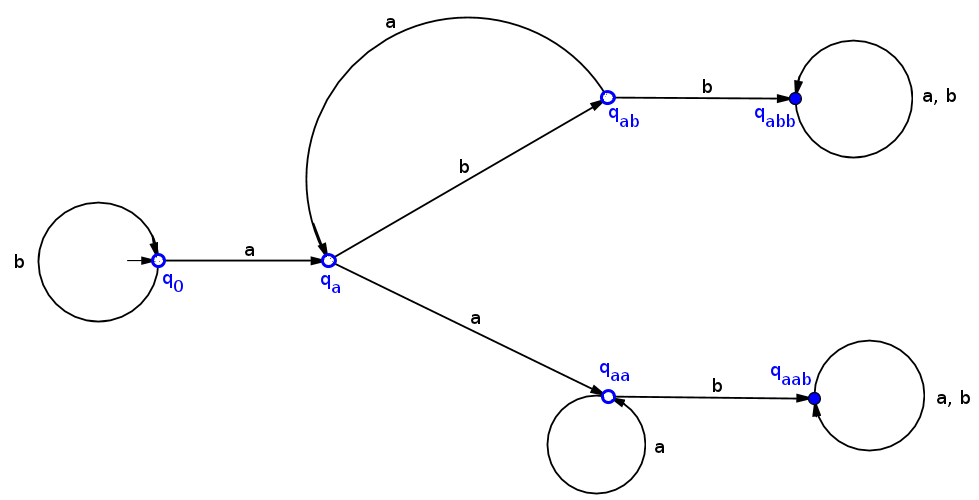
\includegraphics[width = \textwidth]{image-1.png}}

Опишем процесс построения. Сначала "склеим" строки $aab$ и $abb$ в корневое дерево префиксов. Получим ту часть ${\cal A}$, которая состоит из всех его состояний и ребер, которые на диаграмме изображены прямыми отрезками. В состояния $q_{abb}$ и $q_{aab}$ автомат должен переходить после того, как было найдено вхождение подстрок $abb$ и $aab$ соответственно. "Замкнем" эти состояния и сделаем их финальными. После перехода в одно из этих состояний ${\cal A}$ из него уже не выйдет.

Остается только построить ребра, которые соответствуют переходам в состояние, соответствующее концу максимального собственного префикса, совпадающего с суффиксом текущей строки (то есть переход в соответствии со значением префикс-функции). Текущей строкой для любого состояния называется строка, полученная конкатенацией меток ребер вдоль пути от корня до текущей вершины, и буквы, по которой мы в данный момент строим ребро. Так и сделаем.

Вершине $q_{ab}$ соответствует строка $aba$, максимальным собственным префиксом совпадающим с суффиксом которой является $a$. Соответственно проведем ребро с меткой $a$ в вершину $q_a$. Вершине $q_{aa}$ соответствует строка $aaa$, максимальным собственным префиксом совпадающим с суффиксом которой является $aa$. Соответственно проведем ребро с меткой $a$ в вершину $q_{aa}$. Из корня дерева недостающее ребро проведем в корень.

${\cal A}$ корректен и принимает язык $N$ по построению, корректность которого, в свою очередь, следует из корректности КМП (а точнее Ахо-Корасик) алгоритма.

{\bf (ii)}


\medskip

{\bf Задача 2}

{\bf (i)}
Для начала построим следующие автоматы: ${\cal A}_1$ - автомат, принимающий язык $L_1$, все слова которого начинается с $b$, а заканчиваются на $a$; ${\cal A}_2$ - автомат, принимающий язык $L_2$, все слова которого не содержат подслова $bbb$. Эти автоматы изображены диаграмме ниже. Заметим, что построенные автоматы не полные, это облегчит процесс их перемножения.

\centerline{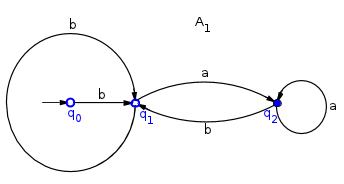
\includegraphics{image-2-a1.png} 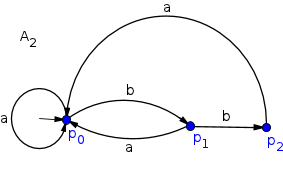
\includegraphics{image-2-a2.png}}

Докажем, что ${\cal A}_1$ принимает $L_1$. Сразу заметим, что ${\cal A}_1$ пустое слово $\eps$ не принимает и далее будем рассматривать слова ненулевой длины. Из начального состояния $q_0$ нет перехода по букве $a$, это означает, что ${\cal A}_1$ может принимать только те слова, которые начинаются с $b$. Остается доказать, что ${\cal A}_1$ может принимать только те слова, которые заканчиваются на $a$. Докажем это индукцией по длине слова $n$. Поскольку после обработки первой буквы слова ${\cal A}_1$ либо останавливается (если слово начинается с $a$), либо переходит в состояние $q_1$ (если слово начинается с $b$), а в состояние $q_0$ больше не возвращается, то при доказательстве будем рассматривать лишь подмножество состояний $\{ q_1, q_2 \}$, считая $q_1$ начальным состоянием. Также, вместо полных слов, начинающихся с $b$, будем рассматривать их суффиксы, длины на 1 меньше, чем длина слова.

{\it База.} Слово $\{ a \}$ длины $n = 1$ принимается ${\cal A}_1$. База доказана.

{\it Переход.} Пусть слова длины меньше $n$, заканчивающиеся на $a$, принимаются ${\cal A}_1$. Докажем, что слова длины $n$, заканчивающиеся на $a$, принимаются ${\cal A}_1$. Возьмем некоторое слово длины $n$. Пропустим через автомат первые $n - 1$ букву. Сейчас ${\cal A}_1$ находится либо в $q_1$, либо в $q_2$. Если $b$ - последняя буква слова, то ${\cal A}_1$ прейдет в $q_1$ и не примет данное слово. Если $a$ - последняя буква слова, то ${\cal A}_1$ прейдет в $q_2$ и примет данное слово. Переход доказан.

Теперь докажем, что ${\cal A}_2$ принимает $L_2$. По построению ${\cal A}_2$ является КДА КМП. Единственное отличие от аналогичного ему ПДКА КМП в том, что отсутствует еще одно состояние, переход в которое осуществлялся бы по букве $b$ из состояния $p_2$. Доказательство его корректности аналогично доказательству корректности автомата из задачи 1.

Теперь построим автомат ${\cal A}_3$, принимающий язык $L_1 \cap L_2 = T$. Для этого воспользуемся конструкцией произведения автоматов $L_3 = L_1 \times L_2$. Поскольку ${\cal A}_1$ и ${\cal A}_2$ не полные, то ${\cal A}_3$ будет иметь всего 4 состояния. Теперь, для того, что бы воспользоваться теоремой 2 необходимо дополнить ${\cal A}_3$ до ПДКА. После этого инвертируем начальноcть / финальность вершин и получим автомат ${\cal A}_4$, принимающий язык $\bar T$. Корректность ${\cal A}_4$ следует из построения. ${\cal A}_3$ и ${\cal A}_4$ изображены на диаграмме ниже.

\centerline{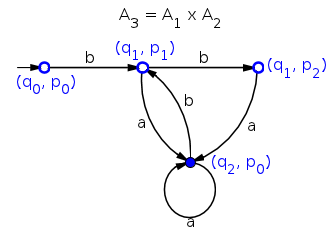
\includegraphics{image-2-a3.png} 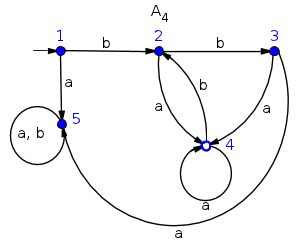
\includegraphics{image-2-a4.png}}

{\bf (ii)}
Пронумеруем состояния автомата ${\cal A}_4$ (на диаграмме выше состояния уже пронумерованы). Теперь, пройдем по приведенному в условии алгоритму в обратном порядке, "раскрывая" соотношения вида $D_{a, b, \{\dots\}}$.
\begin{align*}
  D_{1, 3, \{1, 2, 3\}} &= D_{1, 3, \{1, 2\}} + D_{1, 3, \{1, 2\}} \cdot {D_{3, 3, \{1, 2\}}}^* \cdot D_{3, 3, \{1, 2\}} \\
  {D_{3, 3, \{1, 2\}}}^* &= {\eps}^* = \{ \eps \} \\
  D_{1, 3, \{1, 2\}} &= D_{1, 3, \{1\}} + D_{1, 2, \{1\}} \cdot {D_{2, 2, \{1\}}}^* \cdot D_{2, 3, \{1\}} \\
  D_{1, 3, \{1\}} &= \varnothing \\
  D_{1, 2, \{1\}} &= \{ b \} \\
  {D_{2, 2, \{1\}}}^* &= {\eps}^* = \{ \eps \} \\
  D_{2, 3, \{1\}} &= \{ b \} \\
  D_{1, 3, \{1, 2\}} &= \varnothing + \{ b \} \cdot \{ \eps \} \cdot \{ b \} = \{ bb \} \\
  D_{1, 3, \{1, 2, 3\}} &= \{ bb \} + \{ bb \} \cdot \{ \eps \} \cdot \{ \eps \} = \{ bb \}
\end{align*}

Простой проверкой можно убедиться, что полученное выражение действительно верно.

\medskip

{\bf Задача 5}

Пронумеруем символы в заданной строке:

\smallskip

\noindent
\begin{tabularx}{\textwidth}{|C|C|C|C|C|C|C|C|C|C|C|C|C|C|}
  \hline
  a&b&b&a&b&b&b&a&b&b&a&b&b&b \\
  \hline
  0&1&2&3&4&5&6&7&8&9&10&11&12&13 \\
  \hline
  \hline
  a&b&b&b&a&b&a&b&b&a&b&b&a& \\
  \hline
  14&15&16&17&18&19&20&21&22&23&24&25&26& \\
  \hline
\end{tabularx}

\smallskip

Будем записывать конфигурации $BMA_{aab}$ в следующем виде: $(n, (p, q))$, где $(p, q)$ - соответствует состоянию $BMA_{aab}$ согласно определению из условия, а $n$ - номер символа исходной строки, соответствующего позиции 1-го элемента, видимого в "окошке" $q$.

Последовательность конфигураций $BMA_{aab}$:

\smallskip

\noindent
\begin{tabular}{cccccccc}
  $(0, (3, \#\#\#))$ & $\vdash$ & $(0, (2, \#\#b))$ & $\vdash$ & $(3, (3, \#\#\#))$ & $\vdash$ & $(3, (2, \#\#b))$ & $\vdash$ \\
  $(6, (3, \#\#\#))$ & $\vdash$ & $(6, (2, \#\#b))$ & $\vdash$ & $(6, (1, \#ab))$ & $\vdash$ & $(9, (3, \#\#\#))$ & $\vdash$ \\
  $(9, (2, \#\#b))$ & $\vdash$ & $(9, (1, \#ab))$ & $\vdash$ & $(12, (3, \#\#\#))$ & $\vdash$ & $(13, (3, \#a\#))$ & $\vdash$ \\
  $(13, (1, \#ab))$ & $\vdash$ & $(16, (3, \#\#\#))$ & $\vdash$ & $(17, (3, \#a\#))$ & $\vdash$ & $(17, (1, \#ab))$ & $\vdash$ \\
  $(20, (3, \#\#\#))$ & $\vdash$ & $(20, (2, \#\#b))$ & $\vdash$ & $(23, (3, \#\#\#))$ & $\vdash$ & $(23, (2, \#\#b))$
\end{tabular}

\smallskip

Во время выполнения $BMA_{aab}$ для данной строки, образец ни разу не был найден.

\end{document}
